\documentclass[tikz]{standalone}
\usetikzlibrary{bayesnet, arrows.meta}

\begin{document}
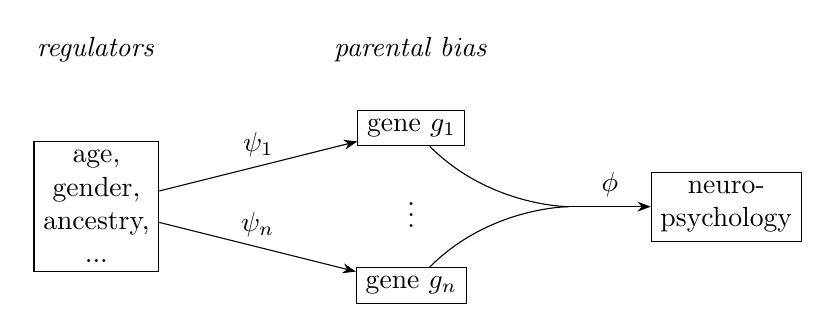
\begin{tikzpicture}[align=center]
\node at (-4,2) {\emph{regulators}};
\node[draw] (A) at (-4,0) {age,\\gender,\\ancestry,\\...};
\node at (0,2) {\emph{parental bias}};
\node[draw] (G1) at (0,1) {gene \(g_1\)};
\node at (0,0) {\vdots};
\node[draw] (Gn) at (0,-1) {gene \(g_n\)};
\coordinate (C) at (2,0);
\node[draw] (B) at (4,0) {neuro-\\psychology};
\draw[-Stealth] (A) -- node[anchor=south] {\(\psi_1\)} (G1);
\draw[-Stealth] (A) -- node[anchor=south] {\(\psi_n\)} (Gn);
\draw[-Stealth] (C) -- node[anchor=south] {\(\phi\)} (B);
\draw (G1) .. controls (1,0) and (2,0) .. (C);
\draw (Gn) .. controls (1,0) and (2,0) .. (C);
\end{tikzpicture}

\end{document}
